\documentclass[11pt,a4paper]{article}

\usepackage[utf8]{inputenc}
\usepackage[T1]{fontenc}
\usepackage[french]{babel}
\usepackage[a4paper,margin=2.4cm]{geometry}
\usepackage{graphicx}
\usepackage{booktabs}
\usepackage{amsmath}
\usepackage{amssymb}
\usepackage{xcolor}
\usepackage{caption}
\usepackage{enumitem}
\usepackage{siunitx}
\usepackage[hidelinks]{hyperref}

\sisetup{
  group-separator={\,},
  group-minimum-digits=4,
  output-decimal-marker={,},
  detect-all,
}

\definecolor{ink}{HTML}{1F2933}
\definecolor{accent}{HTML}{2F6F9F}
\definecolor{warn}{HTML}{C0623D}

\captionsetup{font=small,labelfont={bf,color=ink}}
\setlist{itemsep=2pt,parsep=0pt,topsep=4pt}

\newcommand{\code}[1]{\texttt{\small #1}}

\title{\vspace{-1.5cm}\textbf{Plateforme d'analyse de la performance\\publicitaire Meta}\\[0.3cm]
\large Extraction, entrepôt analytique et diagnostic statistique\\d'un compte Meta Ads}
\author{Rapport de stage --- Ingénierie Informatique, spécialité IA \& Données}
\date{Août 2026}

\begin{document}

\maketitle
\thispagestyle{empty}

\begin{abstract}
\noindent
Ce rapport présente la conception et la réalisation d'une plateforme d'analyse
de la performance publicitaire pour un annonceur du secteur événementiel. Le
travail comprend trois couches~: un extracteur de l'historique de l'API Meta
Marketing conçu pour résister aux limitations de débit et aux interruptions, un
entrepôt analytique local de \num{167144} lignes, et un moteur de diagnostic
statistique appliquant une inférence par bootstrap par grappes avec contrôle du
taux de fausses découvertes.

L'analyse a mis en évidence trois anomalies chiffrées et actionnables, dont un
défaut de suivi des conversions qui empêche l'algorithme d'optimisation de Meta
de fonctionner correctement, et un emplacement publicitaire dont le coût par
conversion est seize fois supérieur à la moyenne du compte. Une analyse du
contenu des publicités établit en outre que les formats qui captent le plus
l'attention sont ceux qui convertissent le moins~: optimiser sur le taux de
clic revient à sélectionner contre la conversion.

Deux hypothèses prédictives ont par ailleurs été testées et écartées, faute de
support dans les données. Le rapport insiste sur les précautions
méthodologiques qui distinguent un résultat d'un artefact, et sur les limites
qui interdisent toute conclusion causale.
\end{abstract}

\vspace{0.5cm}
\tableofcontents
\newpage

% ------------------------------------------------------------------
\section{Contexte et problématique}

\subsection{L'entreprise et son activité publicitaire}

L'entreprise d'accueil commercialise des billets pour des événements culturels
au Maroc --- concerts, festivals, spectacles d'humour --- répartis sur une
dizaine de villes. L'acquisition de clients repose presque intégralement sur la
publicité payante Meta (Facebook et Instagram).

Chaque événement fait l'objet d'une ou plusieurs campagnes publicitaires. Le
volume est important~: sur la période étudiée, \num{106} campagnes, \num{305}
ensembles de publicités et \num{374} publicités distinctes ont été actifs, pour
une dépense totale de \num{42781}~\$.

\subsection{Le problème initial}

Le suivi budgétaire était entièrement manuel. Chaque jour, un membre de
l'équipe relevait dans l'interface Meta les dépenses de chaque campagne pour les
reporter dans un tableur. Ce processus présentait trois faiblesses~:

\begin{itemize}
  \item \textbf{Coût en temps} --- plusieurs heures hebdomadaires de saisie.
  \item \textbf{Latence} --- les écarts entre budget prévu et dépense réelle
        n'étaient constatés qu'après coup.
  \item \textbf{Absence de profondeur} --- seule la dépense agrégée par
        campagne était suivie. Aucune information sur \emph{qui} voyait les
        publicités, \emph{où} elles étaient diffusées, ni \emph{à quel moment}.
\end{itemize}

\subsection{Démarche adoptée}

Une première phase a consisté à automatiser la collecte quotidienne, supprimant
la saisie manuelle. Cette automatisation, opérationnelle, alimente les tableaux
de bord de l'équipe.

Ce rapport porte sur la phase suivante~: transformer cette collecte
opérationnelle en un dispositif d'analyse capable de répondre à la question qui
intéresse réellement l'entreprise --- \emph{où le budget publicitaire est-il mal
employé, et de combien~?}

% ------------------------------------------------------------------
\section{Architecture de la solution}

La plateforme s'organise en trois couches indépendantes, chacune consommant la
sortie de la précédente.

\begin{table}[h]
\centering
\small
\begin{tabular}{@{}llp{7.6cm}@{}}
\toprule
\textbf{Couche} & \textbf{Rôle} & \textbf{Sortie} \\
\midrule
Extraction & Interroger l'API Meta & Fichiers Parquet partitionnés par mois \\
Entrepôt & Rendre les données requêtables & Base DuckDB, vues SQL \\
Analyse & Produire un diagnostic & Classement de segments, rapport \\
\bottomrule
\end{tabular}
\caption{Les trois couches de la plateforme.}
\end{table}

Ce découpage est délibéré. L'extraction est coûteuse et soumise à des quotas~:
elle ne doit être exécutée qu'une fois. L'analyse, en revanche, est relancée
autant de fois que nécessaire sur les données déjà extraites, sans consommer de
quota ni dépendre de la disponibilité de l'API.

% ------------------------------------------------------------------
\section{Couche 1 --- Extraction de l'historique}

\subsection{Pourquoi l'approche naïve échoue}

L'implémentation évidente consiste à boucler sur les jours et à appeler
l'endpoint \code{GET /insights}. Elle s'effondre rapidement~: Meta limite
sévèrement le débit des lectures synchrones, et une extraction sur trois ans
représente plusieurs milliers d'appels.

La méthode retenue est celle que Meta documente pour l'extraction en masse~:
les \emph{tâches asynchrones de rapport}.

\begin{enumerate}
  \item \code{POST /act\_<id>/insights} $\rightarrow$ retourne un
        \code{report\_run\_id}
  \item \code{GET /<report\_run\_id>} $\rightarrow$ interrogation périodique
        jusqu'au statut \code{Job Completed}
  \item \code{GET /<report\_run\_id>/insights} $\rightarrow$ récupération
        paginée des résultats
\end{enumerate}

Le serveur de Meta assume ainsi l'essentiel du travail d'agrégation, et le
nombre d'appels facturés au quota chute d'un ordre de grandeur.

\subsection{Trois propriétés de robustesse}

\paragraph{Temporisation proactive.}
Meta indique la consommation du quota dans les en-têtes de chaque réponse
(\code{x-business-use-case-usage} notamment). Le client les analyse et se met en
pause \emph{avant} d'être bloqué, plutôt que de réagir à une erreur 429 déjà
survenue. Ce point importe particulièrement ici~: le même compte publicitaire
sert simultanément les automatisations de production de l'entreprise, qu'une
extraction gourmande pourrait paralyser.

\paragraph{Reprise sur interruption.}
Une extraction de plusieurs heures \emph{sera} interrompue --- expiration de
jeton, coupure réseau, machine mise en veille. Chaque unité
$(\text{passe},\text{mois})$ terminée est enregistrée immédiatement dans un
fichier de points de reprise. Relancer le programme repart exactement où il
s'était arrêté. Un mois en échec n'est délibérément pas enregistré~: il sera
retenté au lancement suivant, de sorte que l'extraction converge sur plusieurs
exécutions au lieu d'exiger une réussite ininterrompue.

\paragraph{Découpage mensuel.}
Le travail est fractionné par mois calendaire. Les tâches asynchrones restent
assez petites pour que Meta les termine, les points de reprise gagnent une
granularité utile, et des résultats partiels sont exploitables au bout de
quelques minutes.

\subsection{Les cinq passes d'extraction}

\begin{table}[h]
\centering
\small
\begin{tabular}{@{}llrr@{}}
\toprule
\textbf{Passe} & \textbf{Segmentation} & \textbf{Lignes} & \textbf{Part} \\
\midrule
\code{base}       & aucune                                & \num{3643}  & 2{,}2\,\% \\
\code{age\_gender} & âge $\times$ genre                    & \num{43422} & 26{,}0\,\% \\
\code{placement}  & plateforme $\times$ position $\times$ appareil & \num{88497} & 52{,}9\,\% \\
\code{region}     & région                                & \num{6719}  & 4{,}0\,\% \\
\code{hourly}     & heure de la journée                   & \num{24863} & 14{,}9\,\% \\
\midrule
\textbf{Total}    &                                       & \textbf{\num{167144}} & \\
\bottomrule
\end{tabular}
\caption{Volumétrie par passe d'extraction.}
\end{table}

La profondeur du jeu de données ne vient pas de la longueur de l'historique
mais de la \emph{segmentation}~: une même dépense observée sous cinq angles
différents.

% ------------------------------------------------------------------
\section{Couche 2 --- L'entrepôt et le jeu de données}

\subsection{Un entrepôt sans serveur}

Les fichiers Parquet produits par l'extraction sont exposés comme une base
DuckDB. Aucune donnée n'est recopiée~: DuckDB lit les partitions sur place, si
bien qu'une reconstruction après une nouvelle extraction est instantanée et que
les fichiers restent la source de vérité. Le partitionnement de type Hive rend
les clés \code{pass} et \code{month} lisibles comme des colonnes, avec élagage
automatique des partitions.

Ce choix évite d'installer et d'administrer un serveur de base de données pour
un volume qui tient dans 21~Mo, tout en conservant une interface SQL complète.

\subsection{Volumétrie et couverture}

\begin{table}[h]
\centering
\small
\begin{tabular}{@{}lr@{}}
\toprule
Publicités distinctes & \num{374} \\
Ensembles de publicités & \num{305} \\
Campagnes & \num{106} \\
Jours avec activité & \num{65} \\
Dépense totale & \num{42781}~\$ \\
Impressions & \num{73312065} \\
\bottomrule
\end{tabular}
\caption{Caractéristiques du jeu de données extrait.}
\end{table}

\subsection{Une limite majeure~: la concentration temporelle}

L'API Meta conserve environ 37~mois d'historique, et l'extraction a bien
parcouru cette fenêtre complète. Le résultat est cependant très déséquilibré~:

\begin{table}[h]
\centering
\small
\begin{tabular}{@{}lrr@{}}
\toprule
\textbf{Mois} & \textbf{Lignes} & \textbf{Dépense (\$)} \\
\midrule
2023-10 & \num{89}   & \num{253} \\
2026-02 & \num{31}   & \num{20} \\
2026-03 & \num{13}   & \num{0} \\
2026-06 & \num{43}   & \num{106} \\
2026-07 & \num{2249} & \num{29320} \\
2026-08 & \num{1218} & \num{13082} \\
\bottomrule
\end{tabular}
\caption{Répartition mensuelle. Les mois absents ne contiennent aucune donnée.}
\end{table}

\textbf{Plus de 95\,\% des données portent sur juillet et août 2026.} Le compte
publicitaire est resté quasi inactif entre octobre 2023 et juin 2026. On ne
dispose donc pas de trois ans d'historique mais d'environ deux mois d'activité
réelle.

Cette contrainte a été identifiée avant le cadrage analytique, et elle l'a
orienté. Elle écarte définitivement toute modélisation exigeant de la
saisonnalité --- modèle de mix marketing, prévision à long terme, comparaison
d'une année sur l'autre --- et concentre le travail sur ce que deux mois de
données denses et finement segmentées permettent réellement d'établir.

\subsection{Schéma}

Chaque ligne représente une entité (publicité ou campagne) pour un jour donné,
et pour un segment lorsque la passe en définit un.

\begin{itemize}
  \item \textbf{Identité} --- date, identifiants et noms de campagne, ensemble
        et publicité
  \item \textbf{Diffusion} --- impressions, clics, dépense, couverture,
        répétition, CPM, CPC, CTR
  \item \textbf{Entonnoir} --- clic sur lien, vue de page, vue de contenu,
        recherche, ajout au panier, initiation de paiement, achat, et la valeur
        monétaire associée à chacun
  \item \textbf{Engagement} --- vues de vidéo, interactions, commentaires
\end{itemize}

Les compteurs de conversion utilisent un type entier acceptant la valeur nulle,
afin de distinguer \guillemotleft~Meta n'a rien remonté~\guillemotright{} de
\guillemotleft~Meta a remonté zéro~\guillemotright. La distinction est
essentielle pour modéliser un entonnoir. Le contenu brut renvoyé par l'API est
également conservé, de sorte qu'un type d'action non anticipé reste récupérable.

% ------------------------------------------------------------------
\section{Couche 3 --- Méthodologie statistique}

Cette section détaille les choix méthodologiques, car ils déterminent la
fiabilité des résultats de la section suivante.

\subsection{Comparer des taux, non des volumes}

Un segment ayant reçu dix fois le budget d'un autre doit convertir dix fois plus
avant d'être jugé performant. La dépense joue donc le rôle d'exposition, et le
modèle naturel est un taux de Poisson~:

\begin{equation}
  C_i \sim \mathcal{P}\!\left(\lambda_i \cdot s_i\right)
\end{equation}

où $C_i$ est le nombre de conversions du segment $i$, $s_i$ sa dépense, et
$\lambda_i$ son taux de conversion par unité monétaire. L'indice de performance
rapporté dans les résultats est le rapport entre conversions observées et
attendues sous le taux global $\bar{\lambda}$~:

\begin{equation}
  I_i = \frac{C_i}{\bar{\lambda} \cdot s_i},
  \qquad
  \bar{\lambda} = \frac{\sum_j C_j}{\sum_j s_j}
\end{equation}

Une valeur $I_i = 1$ signifie que le segment se comporte exactement comme la
moyenne du compte.

\subsection{Le piège de la surdispersion}

La première implémentation testait $\lambda_i$ contre $\bar{\lambda}$ au moyen
d'un test du score, en corrigeant la surdispersion par un paramètre de Pearson~:

\begin{equation}
  \hat{\phi} = \frac{1}{n-1}\sum_{i}
  \frac{\left(C_i - \bar{\lambda} s_i\right)^2}{\bar{\lambda} s_i}
\end{equation}

Cette approche a produit un résultat incohérent~: $\hat{\phi} = 52$, et plus
aucun segment significatif --- alors même que les intervalles de confiance de
certains segments ne se recouvraient pas.

L'explication est que $\hat{\phi}$ est estimé sur les écarts \emph{entre}
segments, c'est-à-dire précisément sur l'effet que le test cherche à détecter.
Le dispositif s'auto-annulait~: plus les segments diffèrent réellement, plus la
correction gonfle et masque cette différence.

Le paramètre de dispersion reste calculé et affiché à titre de diagnostic, mais
il ne pilote plus la décision statistique.

\subsection{Bootstrap par grappes}

L'inférence repose désormais sur un bootstrap non paramétrique. Le choix de
l'unité de rééchantillonnage est déterminant.

Les lignes sont des observations $(\text{publicité},\text{jour})$~; or les jours
d'une même publicité partagent le même visuel, la même audience et la même
enchère. Ils ne constituent pas des observations indépendantes. Rééchantillonner
les lignes traiterait ces répétitions comme autant de preuves distinctes et
produirait des intervalles beaucoup trop étroits.

Le bootstrap rééchantillonne donc les \emph{publicités} entières, avec remise.
Pour $B$ répliques et un segment comptant $K$ publicités~:

\begin{equation}
  \lambda^{(b)} = \frac{\sum_{k \in \mathcal{S}_b} C_k}
                       {\sum_{k \in \mathcal{S}_b} s_k},
  \qquad
  \mathcal{S}_b \sim \text{Uniforme}(\{1,\dots,K\})^{K}
\end{equation}

Le passage au bootstrap par grappes a élargi les intervalles d'environ 20\,\%,
ce qui correspond à l'effet attendu lorsque l'on cesse de sur-compter des
observations corrélées.

\subsection{Référence par exclusion}

Chaque segment est comparé non pas à la moyenne globale --- qui l'inclut --- mais
au taux agrégé de tous les \emph{autres} segments~:

\begin{equation}
  \lambda_{-i} = \frac{\sum_{j \neq i} C_j}{\sum_{j \neq i} s_j}
\end{equation}

Sans cette précaution, un segment assez gros pour dominer la moyenne se
retrouverait comparé à lui-même, ce qui atténuerait mécaniquement tout écart.

\subsection{Contrôle des fausses découvertes}

Tester 150~segments au seuil $\alpha = 0{,}05$ produit mécaniquement une
poignée de faux positifs. Les valeurs~$p$ issues du bootstrap sont donc
ajustées par la procédure de Benjamini--Hochberg, qui contrôle le taux de
fausses découvertes~:

\begin{equation}
  q_{(k)} = \min_{j \geq k}
  \left\{ \min\left(1, \frac{m}{j}\, p_{(j)}\right) \right\}
\end{equation}

Le contrôle du FDR plutôt que du risque familial est ici le bon compromis~:
l'objectif est une liste restreinte de pistes à instruire, non une garantie
absolue sur chaque élément.

\subsection{Garde-fous}

\begin{itemize}
  \item Un segment doit dépasser \emph{à la fois} un nombre minimal de
        conversions attendues et une part minimale de la dépense totale. Le
        premier seuil protège l'approximation normale~; le second, indépendant
        de l'échelle, écarte les segments dérisoires. Sans lui, un segment
        représentant 1~\$ de dépense ressortait comme significatif sur la
        dimension géographique, où le taux de clics par dollar est élevé.
  \item Les segments exclus sont comptés et signalés, jamais silencieusement
        écartés~: un filtre invisible est un biais invisible.
  \item Les dimensions pour lesquelles Meta ne remonte aucune conversion sont
        traitées en classement seul, sans recommandation budgétaire.
\end{itemize}

% ------------------------------------------------------------------
\section{Résultats}

\subsection{Anomalie critique~: le suivi des achats}

\begin{figure}[h]
\centering
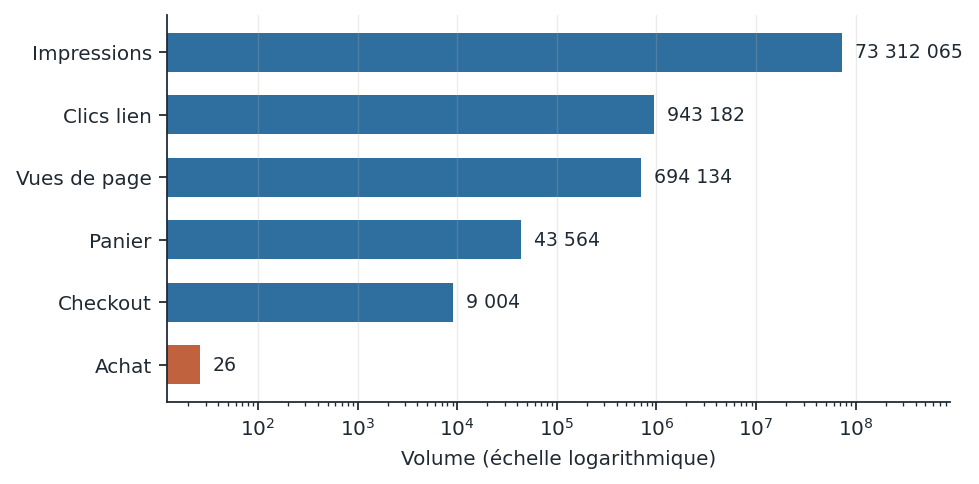
\includegraphics[width=0.86\textwidth]{../figures/funnel.png}
\caption{Entonnoir de conversion complet, échelle logarithmique. La chute
finale est de trois ordres de grandeur.}
\end{figure}

L'entonnoir se comporte normalement jusqu'à l'initiation de paiement, puis
s'effondre~:

\begin{table}[h]
\centering
\small
\begin{tabular}{@{}lrr@{}}
\toprule
\textbf{Étape} & \textbf{Volume} & \textbf{Taux de passage} \\
\midrule
Vues de page de destination & \num{694134} & --- \\
Ajouts au panier            & \num{43564}  & 6{,}3\,\% \\
Initiations de paiement     & \num{9004}   & 20{,}7\,\% \\
\textbf{Achats}             & \textbf{\num{26}} & \textbf{0{,}29\,\%} \\
\bottomrule
\end{tabular}
\caption{Progression dans l'entonnoir sur l'ensemble de la période.}
\end{table}

Un taux de passage du paiement à l'achat se situe habituellement entre 40 et
70\,\% dans le commerce en ligne. La valeur observée est inférieure de deux
ordres de grandeur. Il ne s'agit pas d'un problème commercial mais d'un
\textbf{défaut technique du pixel de suivi}~: l'événement \code{Purchase} ne se
déclenche pas correctement sur la page de confirmation de paiement.

Les conséquences sont lourdes~:

\begin{itemize}
  \item \textbf{L'algorithme de Meta optimise à l'aveugle.} Il ne peut pas
        apprendre à cibler des acheteurs s'il n'en observe que quelques
        dizaines. Les campagnes s'optimisent en pratique sur l'ajout au panier
        ou le trafic, ce qui est nettement moins efficace.
  \item \textbf{Le retour sur investissement affiché est faux}, et toute
        décision budgétaire fondée sur lui est biaisée.
  \item \textbf{Le reciblage des paniers abandonnés} est dégradé.
\end{itemize}

Corriger ce pixel est vraisemblablement l'action à plus fort impact sur
l'ensemble du compte. C'est aussi la moins coûteuse.

En conséquence, toutes les analyses de ce rapport prennent l'initiation de
paiement comme mesure de conversion. C'est l'étape la plus profonde de
l'entonnoir dont le suivi soit fiable, et c'est la pratique usuelle lorsque le
suivi des achats est défaillant.

\subsection{Emplacements publicitaires}

\begin{figure}[h]
\centering
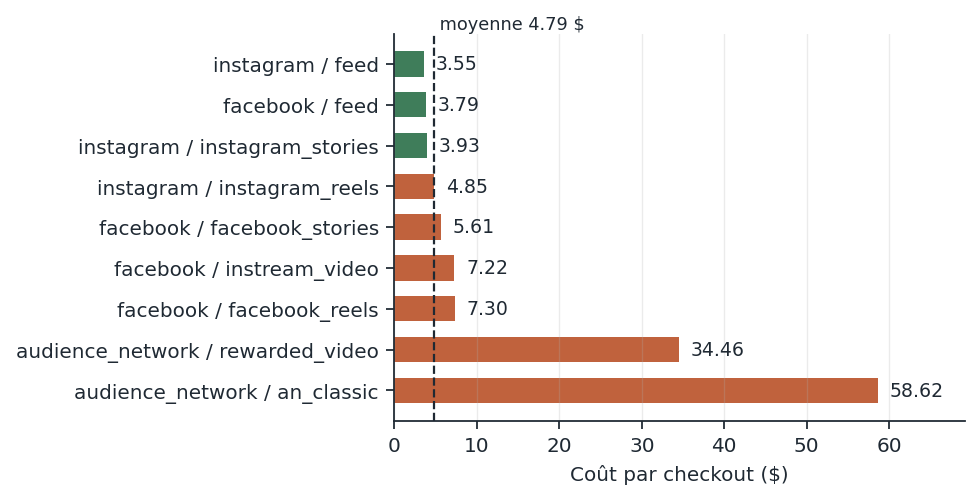
\includegraphics[width=0.88\textwidth]{../figures/placement.png}
\caption{Coût par initiation de paiement selon l'emplacement. En vert, les
emplacements plus efficaces que la moyenne du compte.}
\end{figure}

L'écart entre le meilleur et le pire emplacement est d'un facteur~16.

\begin{table}[h]
\centering
\small
\begin{tabular}{@{}lrrrc@{}}
\toprule
\textbf{Emplacement} & \textbf{Dépense (\$)} & \textbf{Conv.} & \textbf{Coût (\$)} & \textbf{Signif.} \\
\midrule
instagram / feed              & \num{8157}  & \num{2298} & 3{,}55 & oui \\
facebook / feed               & \num{6879}  & \num{1817} & 3{,}79 & oui \\
instagram / stories           & \num{5628}  & \num{1432} & 3{,}93 & oui \\
instagram / reels             & \num{10589} & \num{2181} & 4{,}85 & non \\
facebook / stories            & \num{724}   & \num{129}  & 5{,}61 & non \\
facebook / instream video     & \num{614}   & \num{85}   & 7{,}22 & oui \\
facebook / reels              & \num{6434}  & \num{881}  & 7{,}30 & oui \\
audience network / rewarded   & \num{448}   & \num{13}   & 34{,}46 & oui \\
\textbf{audience network / classic} & \num{3107} & \num{53} & \textbf{58{,}62} & oui \\
\bottomrule
\end{tabular}
\caption{Performance par emplacement. \guillemotleft~Signif.~\guillemotright{}
indique un écart survivant au contrôle du taux de fausses découvertes.}
\end{table}

Deux cibles se dégagent~:

\paragraph{Audience Network.} \num{3555}~\$ dépensés pour un coût par conversion
de 58,62~\$, contre 3,55~\$ sur le fil Instagram. Le réseau d'audience diffuse
sur des applications tierces, où la qualité du trafic est notoirement faible.
Sa désactivation ne demande qu'un réglage et ne comporte pas de contrepartie
identifiable.

\paragraph{Facebook Reels.} \num{6434}~\$, soit 15\,\% du budget, pour un coût
double de celui du fil Instagram. Le cas est moins tranché~: ce format sert
peut-être un objectif de notoriété que la mesure du paiement ne capte pas.
L'écart mérite néanmoins d'être discuté avec l'équipe média.

\subsection{Répartition démographique}

\begin{figure}[h]
\centering
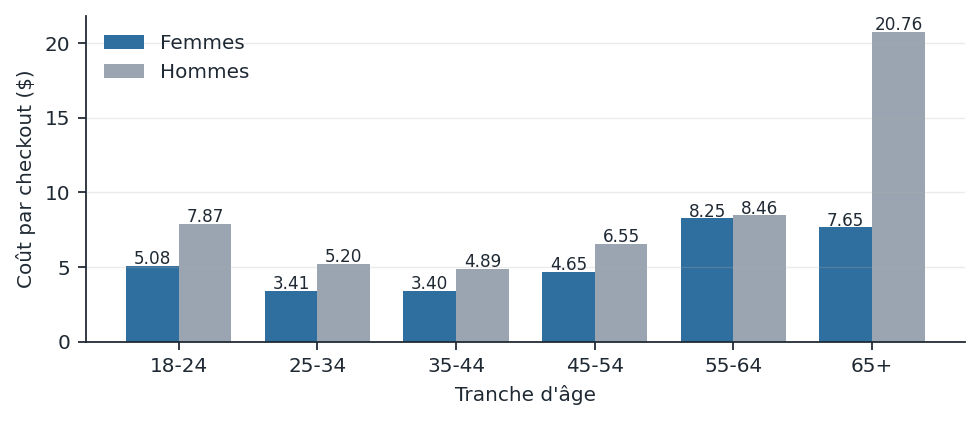
\includegraphics[width=0.86\textwidth]{../figures/demographics.png}
\caption{Coût par conversion par tranche d'âge et par genre.}
\end{figure}

Les segments féminins de 25--34 et 35--44~ans ressortent significativement
au-dessus de la moyenne (indice~1,40 ; $q = 0{,}001$), avec un coût par
conversion de 3,40~\$. Le segment masculin 25--34~ans, qui reçoit pourtant la
dépense la plus élevée du compte (\num{9261}~\$), affiche 5,20~\$.

Globalement, les segments masculins captent 55\,\% du budget pour 45\,\% des
conversions.

\subsection{Répartition horaire}

\begin{figure}[h]
\centering
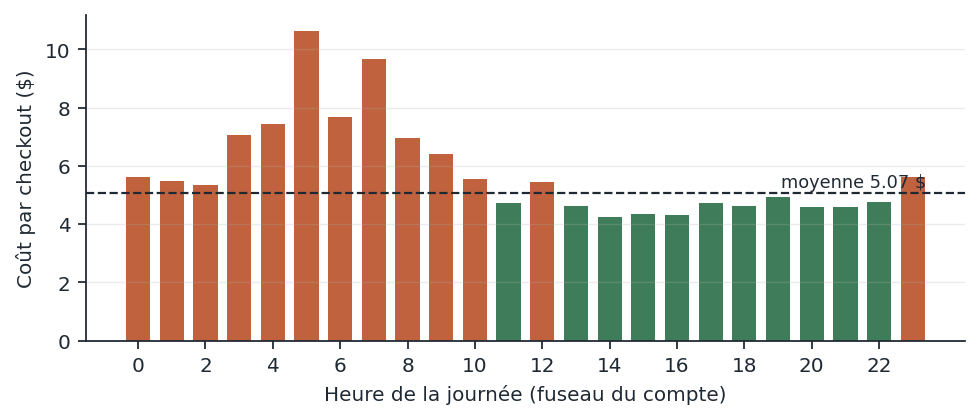
\includegraphics[width=0.88\textwidth]{../figures/hourly.png}
\caption{Coût par conversion selon l'heure de diffusion.}
\end{figure}

Les heures nocturnes, de 3~h à 8~h, présentent un coût significativement
supérieur~: jusqu'à 10,64~\$ à 5~h contre 4,25~\$ à 14~h. Environ \num{2400}~\$
sont dépensés dans cette plage. Une restriction horaire est envisageable, sous
réserve de vérifier que ces heures ne servent pas à capter une audience
spécifique.

\subsection{Simulation de réallocation}

En déplaçant la dépense des segments significativement sous-performants vers
les segments significativement performants, en proportion de leur dépense
actuelle~:

\begin{table}[h]
\centering
\small
\begin{tabular}{@{}lrr@{}}
\toprule
\textbf{Dimension} & \textbf{Plafond linéaire} & \textbf{Estimation saturée} \\
\midrule
Emplacement & $+20{,}4\,\%$ & $+12{,}9\,\%$ \\
Démographie & $+17{,}7\,\%$ & $+10{,}0\,\%$ \\
\bottomrule
\end{tabular}
\caption{Gain de conversions estimé à budget constant.}
\end{table}

Deux bornes sont rapportées plutôt qu'une valeur unique. Le plafond linéaire
suppose que le budget déplacé convertit au taux actuel du segment receveur~:
c'est un majorant certainement optimiste, aucun canal ne conservant son
efficacité lorsque son budget augmente. L'estimation saturée suppose des
rendements décroissants~:

\begin{equation}
  C_{\text{nouveau}} = C_{\text{actuel}}
  \left(\frac{s_{\text{nouveau}}}{s_{\text{actuel}}}\right)^{\alpha},
  \qquad \alpha = 0{,}8
\end{equation}

La valeur $\alpha = 0{,}8$ est une hypothèse issue de la littérature sur les
courbes de réponse publicitaire, non une mesure effectuée sur ces données.

% ------------------------------------------------------------------
\section{Deux hypothèses mises à l'épreuve}

Les résultats précédents sont descriptifs. Cette section rapporte deux
tentatives de modélisation prédictive. Aucune n'a abouti au livrable envisagé,
et les raisons de cet échec sont plus instructives que ne l'aurait été un
modèle bien ajusté.

\subsection{La fatigue créative n'a pas lieu}

\paragraph{L'hypothèse.} Un visuel publicitaire s'épuise~: à mesure que la même
audience le revoit, l'attention décroît, le taux de clic chute et le coût par
conversion se dégrade. C'est un phénomène documenté, et la structure des
données s'y prêtait~: \num{374} publicités, des durées de diffusion allant de 1
à 34~jours, et une censure à droite propre --- les publicités encore actives à
la date d'extraction (figure~\ref{fig:lifetime}). Un estimateur de
Kaplan--Meier suivi d'un modèle à risques proportionnels semblait indiqué.

\begin{figure}[h]
\centering
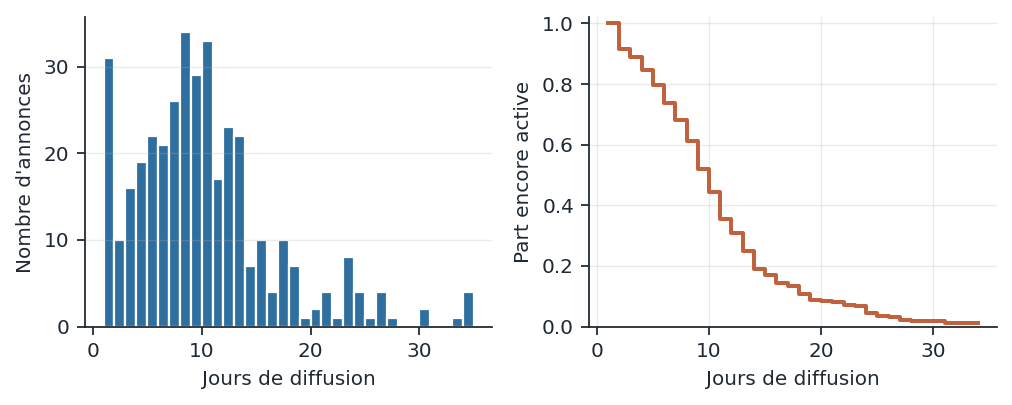
\includegraphics[width=0.92\textwidth]{../figures/lifetime.png}
\caption{Distribution des durées de diffusion et fonction de survie empirique
des \num{374} publicités. La structure convenait à une analyse de survie.}
\label{fig:lifetime}
\end{figure}

\paragraph{Trois tests convergents.} Avant d'ajuster quoi que ce soit, il
fallait vérifier que le phénomène existe.

\begin{figure}[h]
\centering
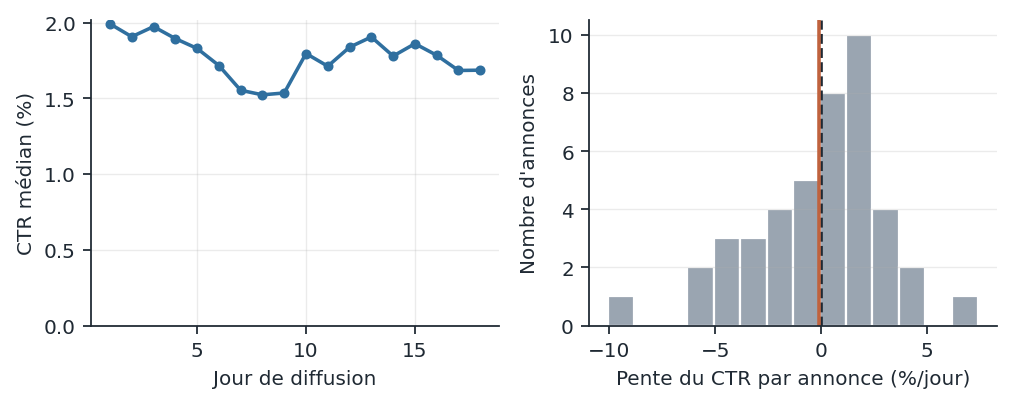
\includegraphics[width=0.92\textwidth]{../figures/fatigue.png}
\caption{À gauche, CTR médian par jour de diffusion sur les 43~publicités
diffusées au moins 12~jours. À droite, distribution des pentes du CTR estimées
publicité par publicité. La ligne pleine marque la pente moyenne et la ligne
pointillée l'absence d'effet~: elles se confondent, ce qui est précisément le
résultat.}
\label{fig:fatigue}
\end{figure}

\begin{enumerate}
  \item \textbf{Profil agrégé.} Sur les 43~publicités diffusées au moins
        12~jours, le CTR médian creuse légèrement vers le septième jour puis
        \emph{remonte}. Aucune décroissance monotone.
  \item \textbf{Régression intra-publicité.} La pente relative du CTR, estimée
        séparément pour chaque publicité, vaut en moyenne
        $-0{,}11\,\%$ par jour et en médiane $+0{,}52\,\%$. Seules 44\,\% des
        publicités déclinent --- soit un tirage à pile ou face. Le test de
        Student contre zéro donne $t = -0{,}23$, $p = 0{,}82$.
  \item \textbf{Le mécanisme manque.} La fréquence quotidienne passe de
        1{,}29 sur les trois premiers jours à 1{,}23 entre le huitième et le
        douzième, puis 1{,}19 au-delà du quinzième. Elle \emph{diminue} au lieu
        de s'accumuler.
\end{enumerate}

\paragraph{Explication.} Le troisième point détermine les deux autres. La
fatigue créative suppose qu'une même personne voie l'annonce de plus en plus
souvent. Or à environ 25~\$ par jour et par publicité, face à une audience
marocaine de plusieurs millions de personnes, le vivier ne sature jamais~:
chaque journée touche une audience largement neuve. Sans exposition cumulée, il
n'existe aucun mécanisme par lequel la fatigue pourrait s'installer.

\paragraph{Pourquoi aucun modèle n'a été ajusté.} Deux voies restaient
ouvertes, toutes deux fautives. Modéliser le \guillemotleft~temps jusqu'à la
fatigue~\guillemotright{} aurait produit une courbe de survie décrivant du
bruit. Modéliser le \guillemotleft~temps jusqu'à l'arrêt~\guillemotright{}
aurait été techniquement valide --- l'événement est réel et observé --- mais
les publicités s'arrêtent parce que le concert a eu lieu ou que l'équipe a
coupé le budget. Le modèle aurait décrit le calendrier des événements en
l'habillant en analyse de survie~: sophistiqué en apparence, vide en substance.

\paragraph{Valeur du résultat négatif.} Il est directement actionnable~:
\textbf{le renouvellement préventif des visuels sur un calendrier fixe n'est
pas justifié sur ce compte}. Cette pratique, standard en achat média et
coûteuse en production, répondrait ici à un problème inexistant.

\subsection{Détection précoce~: un signal réel, un modèle inutile}

\paragraph{La question.} Celle que le media buyer se pose au deuxième jour~:
\emph{cette publicité mérite-t-elle qu'on continue à la financer~?}

\paragraph{Protocole.} Les variables explicatives sont mesurées sur les jours~1
et~2~; la cible --- l'efficacité, en initiations de paiement par dollar --- est
calculée à partir du jour~3. Les fenêtres sont disjointes, aucune observation
ne figure des deux côtés. L'apprentissage porte sur les publicités lancées en
juillet, le test sur celles lancées en août. Le seuil séparant
\guillemotleft~bonnes~\guillemotright{} et \guillemotleft~mauvaises~
\guillemotright{} publicités est la médiane de l'échantillon d'apprentissage,
appliquée telle quelle au test.

\begin{figure}[h]
\centering
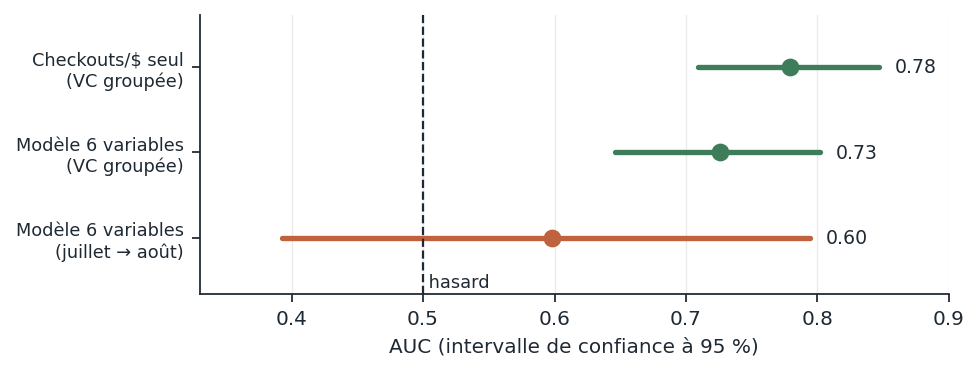
\includegraphics[width=0.9\textwidth]{../figures/early_warning.png}
\caption{Aire sous la courbe ROC selon le protocole d'évaluation, avec
intervalle de confiance bootstrap à 95\,\%.}
\label{fig:earlywarning}
\end{figure}

\paragraph{Résultats.} Trois enseignements, visibles
figure~\ref{fig:earlywarning}.

\emph{Le signal existe.} En validation croisée dont les plis sont groupés par
campagne --- aucune campagne ne figure simultanément en apprentissage et en
test --- l'aire sous la courbe atteint 0{,}73, intervalle $[0{,}65~;~0{,}80]$.
Le hasard est nettement exclu~: les deux premiers jours portent bien de
l'information sur la suite.

\emph{Le modèle est battu par une seule variable.} Le classement par la seule
efficacité précoce atteint 0{,}78, contre 0{,}73 pour la régression logistique
à six variables. Avec \num{174} observations et des variables corrélées, le
modèle ajoute du bruit plutôt que du signal. L'écart entre apprentissage
(0{,}86) et test confirme un sur-apprentissage résiduel malgré la
régularisation.

\emph{La généralisation temporelle n'est pas démontrée.} Sur la séparation
juillet~$\rightarrow$~août, l'aire tombe à 0{,}60 avec un intervalle
$[0{,}39~;~0{,}79]$ contenant 0{,}50. Deux lectures restent possibles --- soit
le signal ne se transporte pas d'un mois à l'autre, soit les 37~publicités de
test ne suffisent pas à le détecter --- et rien dans ces données ne permet de
les départager.

\paragraph{Une limite structurelle.} La corrélation entre efficacité précoce et
efficacité tardive vaut $\rho = 0{,}46$ toutes campagnes confondues, mais
seulement $\rho = 0{,}20$ une fois l'effet campagne retiré. L'essentiel du
pouvoir prédictif distingue les campagnes, non les créatives d'une même
campagne. L'outil convient à l'arbitrage de portefeuille, pas au choix d'un
visuel parmi ses frères --- distinction qu'une aire sous la courbe flatteuse
aurait entièrement masquée.

\paragraph{Le livrable retenu.} Non pas un modèle, mais une règle~:
\textbf{classer les publicités par initiations de paiement par dollar au
deuxième jour et signaler le dernier quartile}. Elle est interprétable,
calculable dans un tableur, ne demande ni réentraînement ni surveillance, et
elle est mesurablement plus performante que le modèle qu'elle remplace.

Un dernier point mérite d'être noté~: le taux de clic ne prédit rien
($\rho = -0{,}10$, aire sous la courbe $0{,}41$). Juger une publicité sur son
CTR --- réflexe courant en achat média --- est trompeur sur ce compte. Seul le
signal de conversion précoce porte de l'information.

% ------------------------------------------------------------------
\section{Ce que la créative explique, et ce qu'elle n'explique pas}

Les sections précédentes mesurent des résultats sans jamais regarder ce qui les
a produits. Cette dernière analyse joint à chaque publicité son \emph{contenu}
--- le texte lu par le spectateur et l'image qu'il a vue --- pour déterminer
quels choix créatifs portent un signal.

\subsection{Extraction et variables}

Les créatives sont récupérées sur une autre arête de l'API, une pagination
classique sans tâche asynchrone. Sur les 360~publicités ayant diffusé, le texte
publicitaire est disponible à 100\,\%, le type d'objet et l'appel à l'action
également, et une vignette a pu être téléchargée pour chacune.

Vingt-et-une variables sont construites~:

\begin{itemize}
  \item \textbf{Texte} (12) --- longueur, nombre de mots, de lignes, d'emojis,
        de mentions, d'exclamations, de questions~; proportion de majuscules~;
        présence d'un marqueur d'urgence, d'un prix, d'une date.
  \item \textbf{Image} (7) --- ratio d'aspect, luminosité, saturation,
        contraste, \emph{colorfulness} au sens de Hasler et Süsstrunk, densité
        de contours, part de pixels sombres.
  \item \textbf{Format} (2) --- vidéo ou image fixe, Reel ou non.
\end{itemize}

Aucun modèle de vision pré-entraîné n'est employé. Avec 360~images réparties
sur 89~campagnes, une représentation profonde fournirait des centaines de
dimensions que les données ne peuvent pas soutenir. Ces variables sont peu
nombreuses, interprétables, et chacune correspond à une décision qu'un
graphiste peut appliquer.

\subsection{L'attention et la conversion s'opposent}

Deux cibles sont modélisées séparément~: le taux de clic, qui mesure
l'attention captée, et les initiations de paiement par dollar, qui mesurent la
conversion obtenue. Le résultat est systématique.

\begin{figure}[h]
\centering
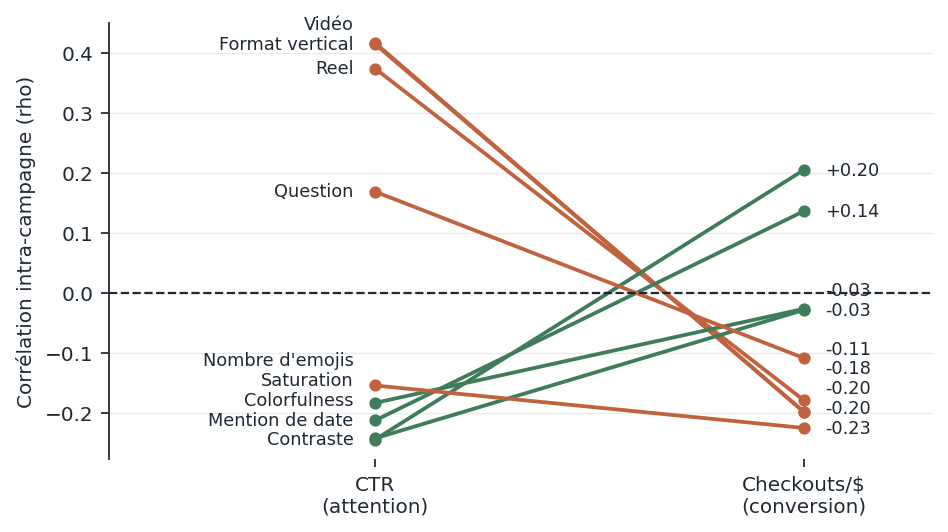
\includegraphics[width=0.86\textwidth]{../figures/creative.png}
\caption{Corrélation de chaque trait créatif avec l'attention (à gauche) et
avec la conversion (à droite), après retrait de l'effet campagne. Les traits
qui gagnent des clics en perdent en conversion, et réciproquement.}
\label{fig:creative}
\end{figure}

Les formats qui captent le plus l'attention --- vidéo, format vertical, Reel
--- sont ceux qui convertissent le moins. Les visuels statiques à fort
contraste font exactement l'inverse. L'ampleur est comparable dans les deux
sens, autour de $|\rho| \approx 0{,}2$ pour la conversion et $0{,}4$ pour
l'attention.

Ces corrélations sont calculées \textbf{après centrage par campagne}. Elles ne
reflètent donc pas le fait que certains événements se vendent mieux que
d'autres~: elles comparent des créatives entre elles, à l'intérieur d'une même
campagne, pour un même événement et une même audience.

\paragraph{Conséquence directe.} Sélectionner les créatives sur le taux de clic
--- réflexe naturel, et la métrique que l'interface de Meta met en avant ---
revient à sélectionner \emph{contre} la conversion. Ce constat complète celui
de la section~7, où l'efficacité précoce prédisait la suite mais où le taux de
clic n'y parvenait pas ($\rho = -0{,}10$). On en connaît maintenant le
mécanisme~: le format pousse les deux métriques en sens opposés.

\subsection{Un confondant qui aurait fait la conclusion}

La corrélation brute la plus forte de toute l'analyse était la proportion de
majuscules dans le texte~: $\rho = -0{,}346$ avec le taux de clic,
$q = 2\cdot10^{-7}$, de loin la plus significative.

Une fois l'effet campagne retiré, elle tombe à $-0{,}129$ et cesse d'être
significative. Sur la conversion, elle passe de $+0{,}239$ à $-0{,}083$~: le
signe s'inverse.

Il s'agissait d'un pur effet de campagne --- certains événements emploient un
style typographique particulier \emph{et} se vendent bien, sans lien de cause à
effet entre les deux. Sans ce contrôle, cette variable aurait constitué le
résultat phare de la section.

\subsection{Capacité prédictive}

\begin{table}[h]
\centering
\small
\begin{tabular}{@{}llcc@{}}
\toprule
\textbf{Cible} & \textbf{Modèle} & \textbf{AUC} & \textbf{IC 95\,\%} \\
\midrule
Attention (CTR) & régression logistique   & 0{,}697 & $[0{,}630~;~0{,}759]$ \\
                & gradient boosting        & 0{,}662 & $[0{,}593~;~0{,}728]$ \\
\addlinespace
Conversion      & régression logistique   & 0{,}603 & $[0{,}534~;~0{,}669]$ \\
                & gradient boosting        & 0{,}616 & $[0{,}547~;~0{,}677]$ \\
\bottomrule
\end{tabular}
\caption{Validation croisée à plis groupés par campagne, 260~publicités
retenues (dépense d'au moins 20~\$).}
\end{table}

La créative explique correctement l'attention et mal la conversion. Le résultat
est cohérent~: ce qui décide de l'achat d'un billet --- l'artiste, la ville, la
date, le prix --- ne se trouve pas dans le visuel. Celui-ci arbitre qui
s'arrête sur l'annonce, pas qui achète.

On notera que le gradient boosting ne surpasse pas la régression logistique,
pour la troisième fois de ce travail. Lorsqu'un modèle non linéaire n'apporte
rien, le plafond tient aux données et non à la classe de modèle.

% ------------------------------------------------------------------
\section{Limites}

Les résultats ci-dessus doivent être lus avec les réserves suivantes.

\paragraph{Nature observationnelle.} Ces données décrivent des allocations que
l'algorithme de Meta a lui-même choisies, en fonction de signaux que le jeu de
données ne contient pas. Qu'un segment convertisse mieux n'implique pas qu'y
transférer du budget produira le même rendement. Seule une expérimentation
contrôlée --- test géographique ou partition d'audience --- peut trancher. Les
simulations dimensionnent l'enjeu et justifient de mener ce test~; elles ne le
remplacent pas.

\paragraph{Profondeur temporelle.} Deux mois d'activité réelle, sur une seule
saison. Aucun effet saisonnier ne peut être estimé, et rien ne garantit que ces
écarts persistent hors de la période estivale.

\paragraph{Mesure de conversion dégradée.} L'analyse porte sur l'initiation de
paiement et non sur l'achat, faute d'un suivi fiable de ce dernier. Si le taux
de transformation du paiement à l'achat varie selon les segments, le classement
s'en trouve biaisé.

\paragraph{Recommandations non littérales.} Certaines conclusions ne sont pas
directement applicables. Le modèle indique par exemple de transférer
\num{22000}~\$ d'Android vers iPhone, ce qui n'a pas de sens opérationnel~:
l'inventaire publicitaire iPhone est fini et ne saurait absorber un doublement
de la dépense. L'écart de performance entre systèmes constitue un signal
directionnel --- il suggère d'examiner l'expérience de paiement sur Android ---
et non une instruction budgétaire.

% ------------------------------------------------------------------
\section{Perspectives}

Quatre prolongements se dégagent, dont deux imposés par les résultats de la
section~7.

\paragraph{Valider expérimentalement.}
C'est le prolongement le plus urgent et le moins coûteux. Toutes les
recommandations de ce rapport reposent sur des données observationnelles. Un
test contrôlé sur Audience Network --- désactivation sur une moitié des
campagnes, maintien sur l'autre, pendant deux semaines --- trancherait
définitivement le cas le plus net, pour un risque budgétaire faible au vu du
coût par conversion actuel de cet emplacement.

\paragraph{Constituer un second jeu de test temporel.}
La question laissée ouverte par la détection précoce --- le signal se
transporte-t-il d'un mois à l'autre~? --- se règlera mécaniquement lorsque
septembre fournira un nouvel échantillon. Le protocole est déjà écrit et
n'aura qu'à être relancé.

\paragraph{Approfondir l'analyse créative.}
La section~8 s'en tient à des statistiques perceptuelles simples, faute d'un
volume permettant une représentation profonde. Avec quelques centaines de
publicités supplémentaires, un modèle de vision fournirait des descripteurs
plus riches --- présence et cadrage du visage de l'artiste, texte incrusté,
type de scène --- dont l'analyse actuelle établit qu'ils mériteraient d'être
mesurés.

\paragraph{Correction du suivi et remesure.}
Une fois le pixel \code{Purchase} réparé, l'ensemble des analyses devrait être
reconduit sur la mesure d'achat réelle, qui est la seule alignée sur l'objectif
commercial.

% ------------------------------------------------------------------
\section{Conclusion}

Ce travail a transformé une automatisation de saisie en un dispositif d'analyse
capable de produire un diagnostic chiffré sur l'emploi du budget publicitaire.

Sur le plan technique, la contribution principale réside moins dans la quantité
de code que dans les choix de robustesse~: extraction asynchrone conforme aux
contraintes de l'API, temporisation proactive préservant les systèmes de
production, reprise sur interruption, et surtout une méthodologie statistique
qui refuse de produire des résultats commodes. La correction du dispositif
d'inférence --- abandon d'une correction de surdispersion qui absorbait le
signal, au profit d'un bootstrap par grappes respectant la structure de
dépendance des données --- illustre cette exigence.

Sur le plan métier, trois constats actionnables ont été établis, dont un défaut
de suivi qui compromet l'optimisation de l'ensemble du compte. La simulation de
réallocation situe le gain potentiel entre 10 et 20\,\% de conversions
supplémentaires à budget constant, sous réserve de validation expérimentale.

La principale limite est la profondeur temporelle des données. Elle a été
identifiée en amont du cadrage analytique, et a conduit à écarter les
approches qu'elle rendait indéfendables plutôt qu'à les mener malgré tout.

\end{document}
